\documentclass[a4paper]{article}
  \usepackage{lipsum}
  \usepackage[margin=1in,left=1.5in,includefoot]{geometry}
  \usepackage{graphicx}

\begin{document}
  \begin{titlepage}
  \begin{center}
  \line(1,0){300}\\
  [.25in]
  \huge{\bfseries MERITS AND DEMERITS OF SOCIAL MEDIA}\\
  [2mm]
  \line(1,0){200}\\
  [1.5cm]
  \textsc{\LARGE bangabandhu sheikh mujibur rahman science and technology university}\\
  [.75cm]
  \textsc{\Large report:  adbantage and disadvantage of social media }\\
  [10cm]
  \end{center}
  
  \begin{flushright}
  \textsc{\huge sakib ahmed}\\
  A General Latex User\\
  18ICTCSE014\\
  january,2020
  \end{flushright}
  \end{titlepage}
  
 %front matter stuff
 \pagenumbering{roman}
 \section*{Summary}
 
Social media refers to the means of interactions among people in which they create, share, and/or exchange information and ideas in virtual communities and networks. The Office of Communications and Marketing manages the main Facebook, Twitter, Instagram, Snapchat, YouTube and Vimeo accounts.

We offer an array of tools, including one-on-one consults with schools, departments and offices looking to form or maintain an existing social media presence to discuss social media goals and strategy, as well as offer insights and ideas. Before creating any social media account, you must submit the Account Request Form. Be sure to check with your school’s communications office for any school specific regulations or branding guidelines.While the tools of social media are easily accessible, the rules of the road are not necessarily intuitive. It’s a new communications landscape, with tremendous opportunities but also a lot to learn.

We developed these guidelines to provide everyone at the university—from communications professionals to department administrators—with basic guidance on how to best use social media toward communications goals, both as the owner of an account and as a user/contributor. The suggestions and best practices outlined here can help you use these channels effectively, protect your personal and professional reputation, and follow university guidelines. We also hope that these guidelines spark conversations among social media practitioners on campus to learn from each other as we explore these emerging platforms.
\begin{figure}[h]
\centering
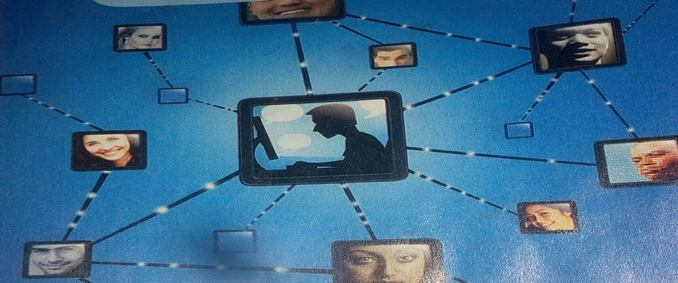
\includegraphics{dmsm}
\caption{Social media}
\end{figure}

 \cleardoublepage
  
  %table of contents
  \tableofcontents
  \thispagestyle{empty}
  \cleardoublepage
  
  %main body stuff
  \pagenumbering{arabic}
  \setcounter{page}{1}  
  
  \section{ YOU REACH LARGE AUDIENCES}
There are millions of people using social media platforms. It’s a great opportunity for your business to reach a large pool of people that are interested in your products or services.

According to Pew Research Center, these are the percentages of U.S. adults that use social media sites online or on mobile:
 \begin{itemize}
  \item YouTube: 73 percent
  \item Facebook: 68 percent
 \item Instagram: 35 percent
 \item Pinterest: 29 percent
 \item Snapchat: 27 percent
 \item LinkedIn: 25 percent
 \item Twitter: 24 percent
 \end{itemize}
 U.S. adults use many of these sites, which creates great opportunities for your business to reach leads. You have numerous opportunities to reach leads and can engage them on these different platforms.
 \begin{figure}[h]
 \centering
 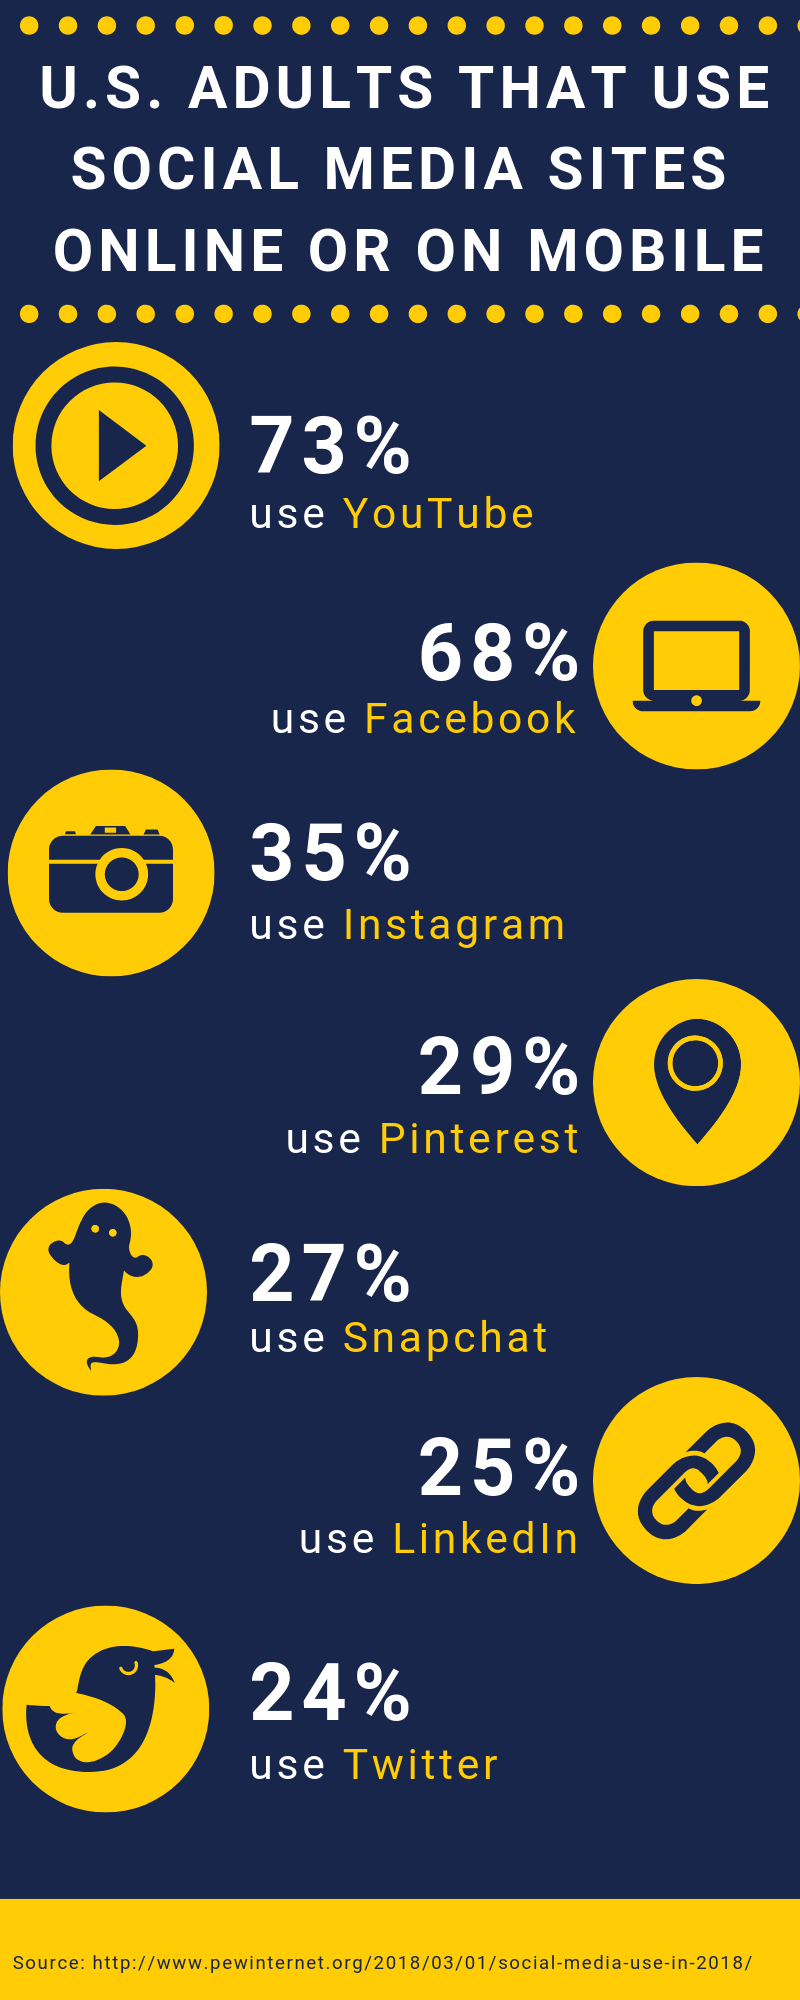
\includegraphics[width=2.5in,height=2.5in]{sa}
 \end{figure}
 \section{ YOU HAVE A DIRECT CONNECTION WITH YOUR AUDIENCE}
 Social media is one of the few marketing strategies that allow you to connect directly with your audience. You know who is interested in your business because they choose to follow your social media account.

This social media advantage helps your business in numerous ways:
 \begin{itemize}
    \item You get to know them better: When you know your audience better, you can deliver more valuable content to them. You make the content more personalized to their interests, which leads to more engagement on your page and with your business.
    \item You provide better customer service: A direct connection with your audience allows you to resolve issues easier. You can address them personally, deal with their issues 1-on-1, and build your brand in a positive light in the process.
    \item You gain valuable insight about your customers: The direct connection with your audience helps you get to know your audience better. You see who interacts with your posts and how they interact with them. It helps you adapt your strategy to make it better for your followers.
    \item You see how your audience perceives your business: It’s always good to know how others view your business. With social media marketing, you know what your audience thinks of your company. It’s a huge advantage of social media marketing because you can capitalize on aspects people like about your business and fix elements they don’t like.
  \end{itemize}
  The direct connection with your audience is a great way to improve your overall marketing campaign. You’ll get insight from your followers and be able to adapt your social media strategy better to meet their needs.
\lipsum[1]
  \newpage
  \section{ YOU CAN CREATE ORGANIC CONTENT}
The ability to post organic content for free is an incredible benefit of social media for business. This opens many opportunities for your company to connect with valuable leads at no cost. It’s one of the reasons why companies love using these platforms.

You can post as much content as you want to engage your audience too.

These platforms enable you to post photos, videos, and more, depending upon the social media network. It’s a great way to put your brand out in front of people interested in your business and help them get more familiar with it.
 
 
  \section{ YOU HAVE ACCESS TO PAID ADVERTISING SERVICES}
If you want to go beyond organic posting, there is an option to run paid advertisements. Each social platform offers its own form of paid advertising. Your social media advertising capabilities will vary depending upon your platform.
Paid advertisements offer your business the opportunity to connect with interested leads that haven’t found your business yet. Social media platforms allow you to tailor your ads to appear in the feeds of people who are looking for your products and services.

This creates a great opportunity for your business to expand your reach and obtain new leads. You help more interested leads find your business, which results in new followers, as well as conversions for your bussiness.
   \newpage
  \section{YOU BUILD YOUR BRAND}
One advantage of social media marketing is the ability to build your brand. When you connect with interested leads, you expose them to your brand. The ability to post organic content for free allows you to build brand recognition repeatedly with your audience.

This builds brand loyalty. The more people get exposed to your brand, the more they become familiar with it. Brand familiarity leads to more conversions down the line because people tend to buy from brands they know well.
Social media also helps you build your brand because it enables sharing. You can share, retweet, and re-pin content on these platforms. This means that followers can share your content with their friends and family, which helps expose your brand to more people.

It’s an excellent way for you to gain new leads. You can reach leads that you wouldn’t reach otherwise. It helps you grow your followers and earn more leads.
 
  
  \section{ YOU DRIVE TRAFFIC TO YOUR WEBSITE}
 Social media is a great catalyst for driving traffic to your business’s website.

Most social media platforms allow you to post content with a link to your website. When you create compelling content, you can entice your audience click on the link. This directs them to your site, where they can learn more about your business.

It’s a great opportunity for you to help your audience get more familiar with your business.

They can check out your website and learn about your products and services.

Depending on your business, you can even let people use your site to book appointments or pay bills. A dental social media marketing strategy, for example, may direct people to the practice’s website to book their first appointment and complete any new patient forms.

More traffic on your site also helps your other marketing efforts because you’ll drive more relevant traffic to your page.

7. YOU CAN EVALUATE YOUR PERFORMANCE
The last advantage to social media marketing is the ability to assess your performance. Whenever you run a marketing campaign, you want to know how it’s performing. Social media platforms make it easy for you to track your campaign to see if you’re driving valuable results.

A social media benefit is you can access informative metrics
You can determine how many people see your posts, comment, like, share, and more. If you run an advertising campaign, you can view metrics for that, too. You’ll see metrics like impressions, clicks, and conversions.

When you can evaluate your social media strategy’s performance, you can optimize it and improve it to drive better results.
  
  \newpage
  
  \section{. YOU CAN JOIN SOCIAL MEDIA NETWORKS FOR FREE}
 One of the biggest advantages of social media marketing is that it is entirely free to start. None of the largest platforms have signup fees of any sort, so the only investment you’ll need to make is in the form of time.

That being said, there are paid advertising options on most social media platforms. These can be a great tool for growing your following and reaching more users, but are by no means mandatory for businesses.
  
 \section{ YOU CAN CREATE VIRAL CONTENT}
Perhaps the most unique advantage of social media is the ability to get help from your followers. People love to share things with their networks, from photos and recipes to interesting articles and hot deals.
\begin{figure}[h]
\centering

\includegraphics[width=4.5in,height=3in]{as}
\end{figure}

Unlike other forms of Internet marketing, like your site and paid advertisements, content on social media is often shared. However wide your reach, your followers can share with their followers, who then share with their followers, giving you a wider reach (with lower cost) than a traditional marketing campaign.
  \newpage
  \section{YOU CAN UNCOVER VALUABLE INSIGHTS}
 You can also use social media to gain valuable information about your customers that will help you make smarter business decisions. For example, social listening allows you to discover how people feel about your company and brand. With social listening, you can uncover conversations about your business and answer questions about your offerings.

What do people like about your business? How can you improve your products and services to better meet the needs of your target audience? Understanding the answers to these questions can your business stand out from the competition and reach more people.
 \section{What are the disadvantages of social media?}
With any marketing strategy, there are always disadvantages. The disadvantages don’t mean that the approach isn’t effective, but rather, present potential hurdles you may have to jump through during your campaign.
\begin{figure}[h]
\centering
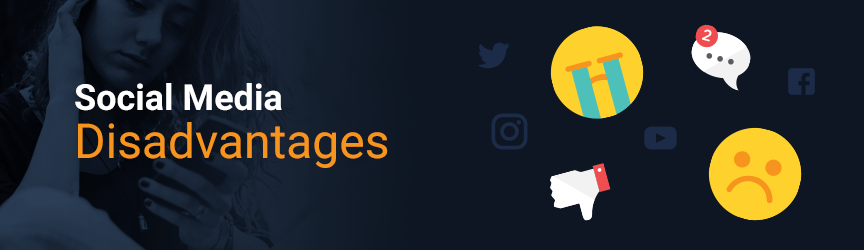
\includegraphics[width=5in,height=5in]{sab}
\caption{}
\end{figure}
Here are four downsides to social media:
 \subsection{ YOU CAN RECEIVE NEGATIVE FEEDBACK}
 People use social media to post content they love, but they also use it to share experiences they didn’t love. If someone had a poor experience with your business, it opens a door of opportunity for them to share their poor experience with others.

This negative feedback comes in different forms. On platforms like Facebook, someone can leave a negative review on your page and share their negative experience. When someone checks out your business next, they’ll look at the reviews and see the negative feedback.

On sites like Twitter, users can tag a company in their posts and share their negative experience. People can retweet that poor experience and spread it across the network.
 \begin{figure}
 \centering
 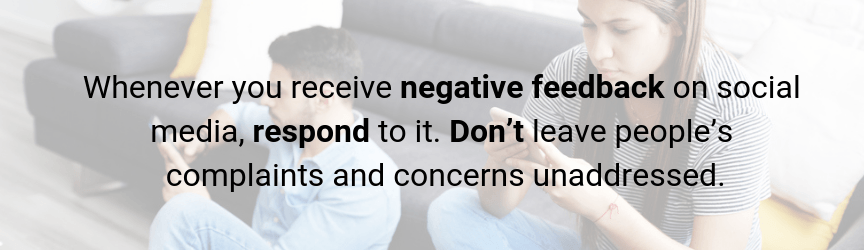
\includegraphics[width=5in,height=4in]{asb}
 \caption{respond-to-feedback-on-social}
 \end{figure}
 Social media platforms are catalysts for complaining and leaving negative feedback. People use their profiles to help others understand their poor experience. Many people feel there is a social obligation to share their experience to prevent others from having the same experience.

Having too much negative feedback can negatively impact your future marketing efforts.

People trust others to give them insight into your company, especially if it’s the first time they are hearing of your business. With social media, it’s possible that negative feedback can hinder your business from earning leads.
  \subsection{How to adapt to this social media disadvantage}
  Whenever you receive negative feedback on social media, respond to it. Don’t leave people’s complaints and concerns unaddressed. Not everyone is going to have a positive experience with your business, but addressing the issues can speak volumes about your company and its values.
  \subsection{YOU OPEN UP THE POTENTIAL FOR EMBARRASSMENT}
  It’s easy for posts to go viral on social media. People keep a close eye on the good and the bad on social media. If you aren’t careful about the content you post, you can end up embarrassing your company and getting caught in an awkward situation.

For example, at one point, the hashtag “WhyIStayed” was trending on social media. This hashtag was about victims of domestic violence sharing their story. The hashtag took social media by storm and became a facilitator for conversations about abusive relationships.
This was an embarrassing moment for DiGiorno that blew up over social media. They spent the next few weeks doing damage control and addressing their mistake with thousands of people on Twitter. The carelessness of the tweet made people have a negative perception of DiGiorno.

When you post on social media, there is always an opportunity to embarrass your business on accident. This is a big downside to social media.
 How to adapt to this social media disadvantage: Always do your research before posting content on social media. Whether it’s a photo, a hashtag, or a video, do your research to see if there is any way it could be construed the wrong way. Research helps you adapt your content to prevent your company from embarrassment.
  \subsection{ YOU MUST SPEND A LOT OF TIME ON YOUR CAMPAIGNS}
 Social media isn’t a one and done type of marketing method. You must constantly create new content, post content, and engage with your audience on these platforms. A big drawback to social media is that it is time-consuming for companies.
 \begin{figure}
 \centering
 
\includegraphics[width=5in,height=4in]{aa}
 \caption{why-use-social-media}
 \end{figure}
 If you have a small business, small marketing department, or limited resources, it’s challenging to manage a social media marketing campaign.

You have to find time to balance posting content, monitoring that content, responding to people, and measuring your content’s impact. If you don’t have the resources, it can be an overwhelming task.

If you aren’t doing enough with your social networks because you don’t have time, people, or programs to help you run your marketing strategy, your campaigns will suffer. You won’t be as effective as someone who has the necessary aspects to run a successful social media campaign.
\begin{figure}
\centering
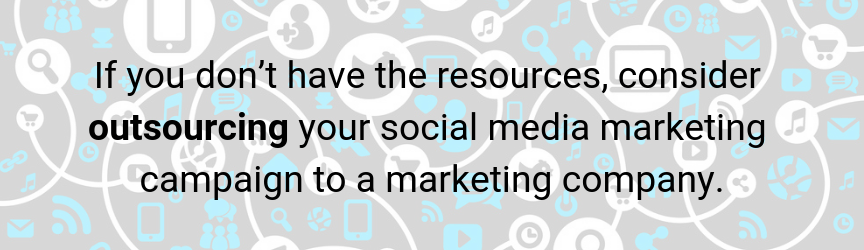
\includegraphics[width=5in,height=4in]{ss}
\caption{use-social-media-marketing-company}
\end{figure}
How to adapt to this social media disadvantage: If you don’t have the resources, consider outsourcing your social media marketing campaign to a social marketing company. You can hire a social media marketing company to handle your campaign for you while you run your business. Not to mention, you’ll partner with people who have years of experience running campaigns and know how to drive success!
  \subsection{YOU HAVE TO WAIT TO SEE RESULTS}
 When companies invest in marketing strategies, they want to see immediate results. You want to know that your strategies are working and that the investment is worth your time. With social media marketing, you don’t see immediate results.

Social media marketing’s success is predicated on the campaign’s overall success. Posting one piece of content doesn’t determine the success of your campaign. You must post multiple pieces of content over a period of time to determine the true success of your campaign.

This is a downside of social media because you have to wait to see results. You must be patient and wait a few weeks to see results before you can adjust your campaign.

How to adapt to this social media disadvantage: The only true adaptation for this downfall is to be patient. You must remind yourself that you can’t see true immediate results until your campaign is running for some time. The best thing you can do is track the performance of your social media posts as you post them to have them ready for comparison once your campaign is running for some time.
\end{document}